


In order to create a basis for the engine choice, a trade study was performed on the engines of similar aircraft. These aircraft, such as the Boeing 777-300, Airbus A330-300, Airbus A330-900, and Airbus A350 XWB, have a similar passenger capacity as the one required in the design competition, however all have a much higher range capability. The primary drivers for the design of the propulsion system are the power requirement for the aircraft, as well as reliability. Since the aircraft will be used as a high capacity transport for a short mission duration, it is vital that the engines can withstand a constant cycle of maximum take off thrust at a higher interval than traditional engines which experience a longer flight duration. Similarly, an engine which may be oversized can be considered and then de-rated in order to increase engine life span, thereby decreasing long term cost.

\subsection{Engine Comparisons}

The following engines, seen below, are used in similar aircraft with great success: Pratt \& Whitney PW4000, General Electric GE90-115B, Rolls-Royce Trent XWB, and Rolls-Royce Trent 7000.

\begin{table}[!h]
    \centering
        \caption{Comparison of Engines on Similar Aircraft}
    \begin{tabular}{|c||c|c|c|c|}\toprule
         & \textbf{PW4000} & \textbf{GE90-115B} & \textbf{RR Trent XWB} & \textbf{RR Trent 7000} \\\hline \hline
         \textbf{Aircraft} & Airbus A330-300 & Boeing 777-300 & Airbus A350 XWB & Airbus A330-900\\ \hline
         \textbf{Maximum Takeoff Thrust [lb]} & 52,000 - 62,000 \cite{PW} & 110,000  \cite{ge90} & 84,200  \cite{xwb} & 71,110  \cite{butterworth}\\ \hline
         \textbf{Dry Weight [lb]} & 12,900  \cite{FAApw} & 19,316  \cite{ge90} & 16,043  \cite{xwb2} & 10,550 \cite{butterworth} \\ \hline
         \textbf{Cost per Unit [USD]} & - & \$ 27.5 million \cite{gecost} & - & \$ 11 million \cite{butterworth} \\ \hline
         \textbf{Bypass Ratio} & 4.9 : 1 \cite{PW} & 9 \cite{safran} & 9.6 : 1 \cite{xwb} & 4.89 : 1 \cite{butterworth} \\ \hline
         \textbf{Fan Diameter [in]} & 94 \cite{PW} & 128 \cite{ge} & 118 \cite{xwb} &  97 \cite{butterworth}\\ \hline
         \textbf{SFC [lb/lbf/hr]} & 0 & 0.545 \cite{butterworth} & 0 &  0.565 \cite{butterworth} \\ \hline
         \textbf{Thrust to Weight} & 4.80-4.03 & 5.69 & 5.24 & 6.74 \\ \bottomrule
    \end{tabular}
    \label{tab:enginecomp}
\end{table}


While the aircraft are similar in capacity, the range on these aircraft is much higher than what is required for the SAM Mk I. As such, an assumption is made that the engines chosen for these aircraft may not be as reliable as necessary for the SAM Mk I, since the engine for the SAM Mk I will experience higher intervals and much more frequent cycling of maximum thrust, leading to more fatigue to the engine. 

In order to validate the choice of a turbofan engine, which was also the type of engine of choice for the similar aircraft compared above, Figure \ref{PropSelection} was used along with the Mach number the SAM Mk I will fly at cruise conditions, 0.775. This figure was used to quickly determine which propulsion systems are overpowered for the flight conditions that the aircraft will fly and rule out which propulsion systems would not be able to meet the flight conditions \cite{raymer}.

\begin{figure} [h!]
    \centering
    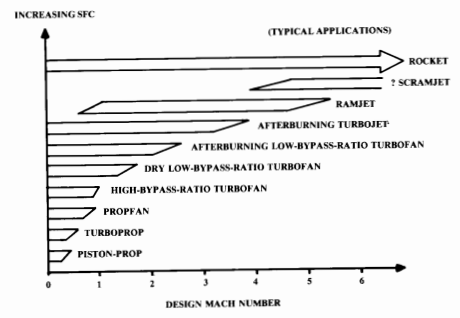
\includegraphics[width=0.8\textwidth]{Photos/PropSelection.PNG}
    \caption{Propulsion System Speed Limits}
    \label{PropSelection}
\end{figure}

\newpage
With a Mach number of 0.775, both piston-prop and turboprop engines are not able to meet the speed requirement for cruise. The propfan propulsion system, while it may be able to handle a Mach number of 0.775, is not ideal as it is operating at the end of its limit. Scramjet and ramjet propulsion systems are overpowered for the SAM Mk I system, leaving only three classes of turbofan engines and an afterburning turbojet engine. According to Raymer, the propulsion system should be one which the lowest on the chart for the specified Mach number, which for this case is the high-bypass-ratio turbofan \cite{raymer}. In addition, all of the engines listed in Table \ref{tab:enginecomp} are high-bypass-ratio turbofan propulsion systems as well, which gives confidence in the high-bypass-ratio turbofan engine being the propulsion system of choice for the SAM Mk I.

\subsection{Engine Requirements}

Using the sizing analysis in which a similar aircraft was seeded into, several of the specifications of the SAM Mk I were inputted in order to obtain a thrust requirement for the aircraft. The sizing analysis estimated that the SAM Mk I would require a thrust of 151,000 lb.

Furthermore, an engine with high reliability was sought after due to the high cycling behaviour of take-off that this aircraft will see. Therefore, an engine which has already undergone certification and has been in service with a proven track record of reliability was prioritized. When accounting for engine de-rating, an engine which may seem overpowered will actually have long term cost savings due to the increase of the engine's lifespan and decrease in maintenance cycle.

In accordance with 14 CFR \S25.903, any engine used on an aircraft must have a type certificate \cite{cfr}. Due to the fact that all of the aforementioned engines are currently in use by commercial aircraft, all engines considered are compliant. 

\subsection{Engine Selection}

The engine of choice for the SAM Mk I will be General Electric's GE90-115B. The selection of this engine was driven by the desire to have an engine that is already in service and has a proven track record of reliability.

\begin{table}[!h]
    \centering
        \caption{GE90-115B Specifications}
    \begin{tabular}{|c||c|}\toprule
         & \textbf{GE90-115B} \\\hline \hline
         \textbf{Maximum Continuous Thrust [lb]} & 110,000  \cite{ge90} \\ \hline
         \textbf{Take-off Thrust (5 minutes) [lb]} & 115,540  \cite{ge90} \\ \hline
         \textbf{Dry Weight [lb]} & 19,316  \cite{ge90}  \\ \hline
         \textbf{Cost per Unit} &  \$ 27.5 million \cite{gecost}  \\ \hline
         \textbf{Bypass Ratio} & 9 \cite{safran}  \\ \hline
         \textbf{Fan Diameter [in]} & 135 \cite{ge} \\ \hline
         \textbf{Engine Length [in]} & 286.7 \cite{ge} \\ \hline
         \textbf{Engine Width [in]} & 148.4 \cite{ge} \\ \hline
         \textbf{Engine Height [in]} & 154.6 \cite{ge} \\ \hline
         \textbf{Thrust to Weight} & 5.69 \\ \bottomrule
    \end{tabular}
    \label{tab:GE90}
\end{table}

The unit cost for this engine was approximately \$27.5 million dollars in 2011 \cite{gecost}. When accounting for inflation, the current price is \$31.5 million dollars. Assuming an average rate of inflation of 3\% a year, the estimated cost of this engine once the SAM Mk I goes into service in 2029 will be approximately \$ 47 million dollars. While the initial cost of the GE90-115B is high, since it is in use on aircraft in 2020, it is possible to refurbish a GE90-115B from a retired aircraft, thereby decreasing the initial cost by using a used engine. Additionally, buying engines in bulk for production will decrease the unit cost of each engine. Additionally, according to Epstein the engine has a propulsive efficiency of approximately 70\% \cite{epstein}.

\begin{figure} [h!]
    \centering
    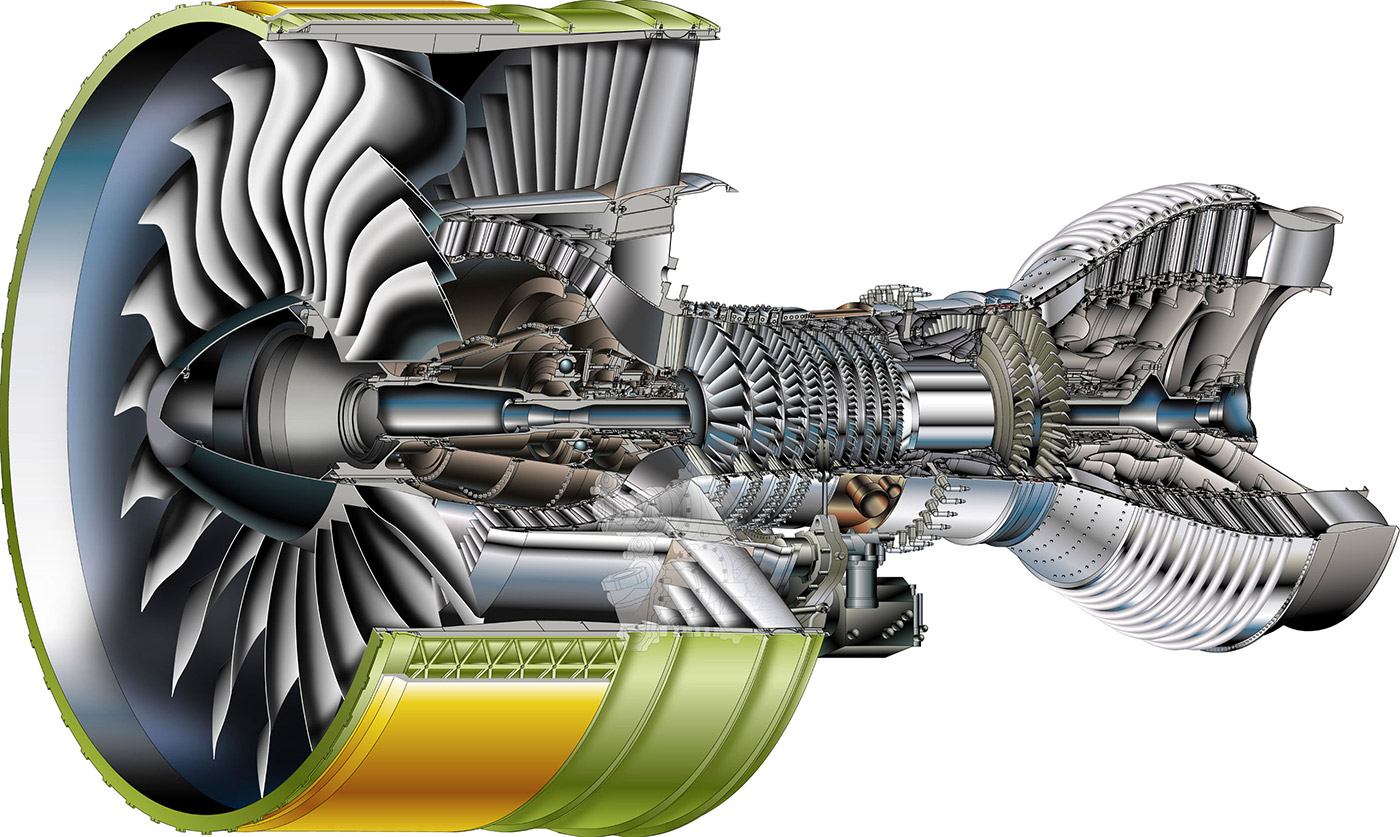
\includegraphics[width=0.8\textwidth]{Photos/ge90cross.jpg}
    \caption{Cross-section of the GE90-115B}
    \label{fig:GeCross}
\end{figure}

The GE90-115B is a dual rotor, high bypass ratio turbofan. It has a 9 stage high pressure compressor that is followed by a 2 stage high pressure turbine. Continuing, a 6 stage low pressure turbine drives the 4 stage low pressure compressor as can be seen in Figure \ref{fig:GeCross} \cite{gecross}. This engine had the first ever composite fan blades in commercial aviation that allowed it to be one-third the weight of industry standard titanium blades at the time. It is also quieter and more efficient than most other engines in its thrust class \cite{ge90}.

The GE90-115B has its gearbox located on the underside of the wing where all other engine accessories such as fuel pumps, oil pumps, and engine control boxes are stored as well. Although no sources have confirmed this location, according to Raymer, it is the most likely location of the the accessory package \cite{raymer}.

\subsection{Validation of Engine Choice}

Since the GE90-115B engine is rated to approximately 110,000 lbs of thrust per engine, in case of an engine-out failure, the engine would still be able to provide more than 70\% of the estimated required thrust in order to keep the plane in flight. This offers an extra level of safety than if a lesser thrust rated engine was chosen which would not be able to provide such a high percentage of necessary thrust. Furthermore, the GE90-115B has a very strong safety record, with it having a reported in-flight shutdown rate of one per million engine flight hours \cite{geifsd}. 

\begin{figure} [h!]
    \centering
    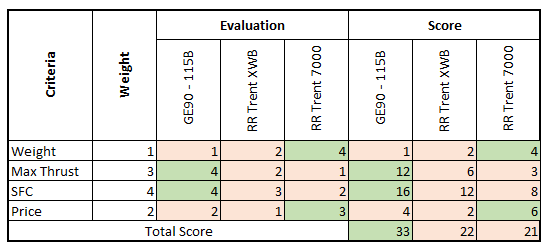
\includegraphics[width=\textwidth]{Photos/GE90Trade.PNG}
    \caption{Engine Trade Study}
    \label{fig:enginetrade}
\end{figure}

\begin{figure} [h!]
    \centering
    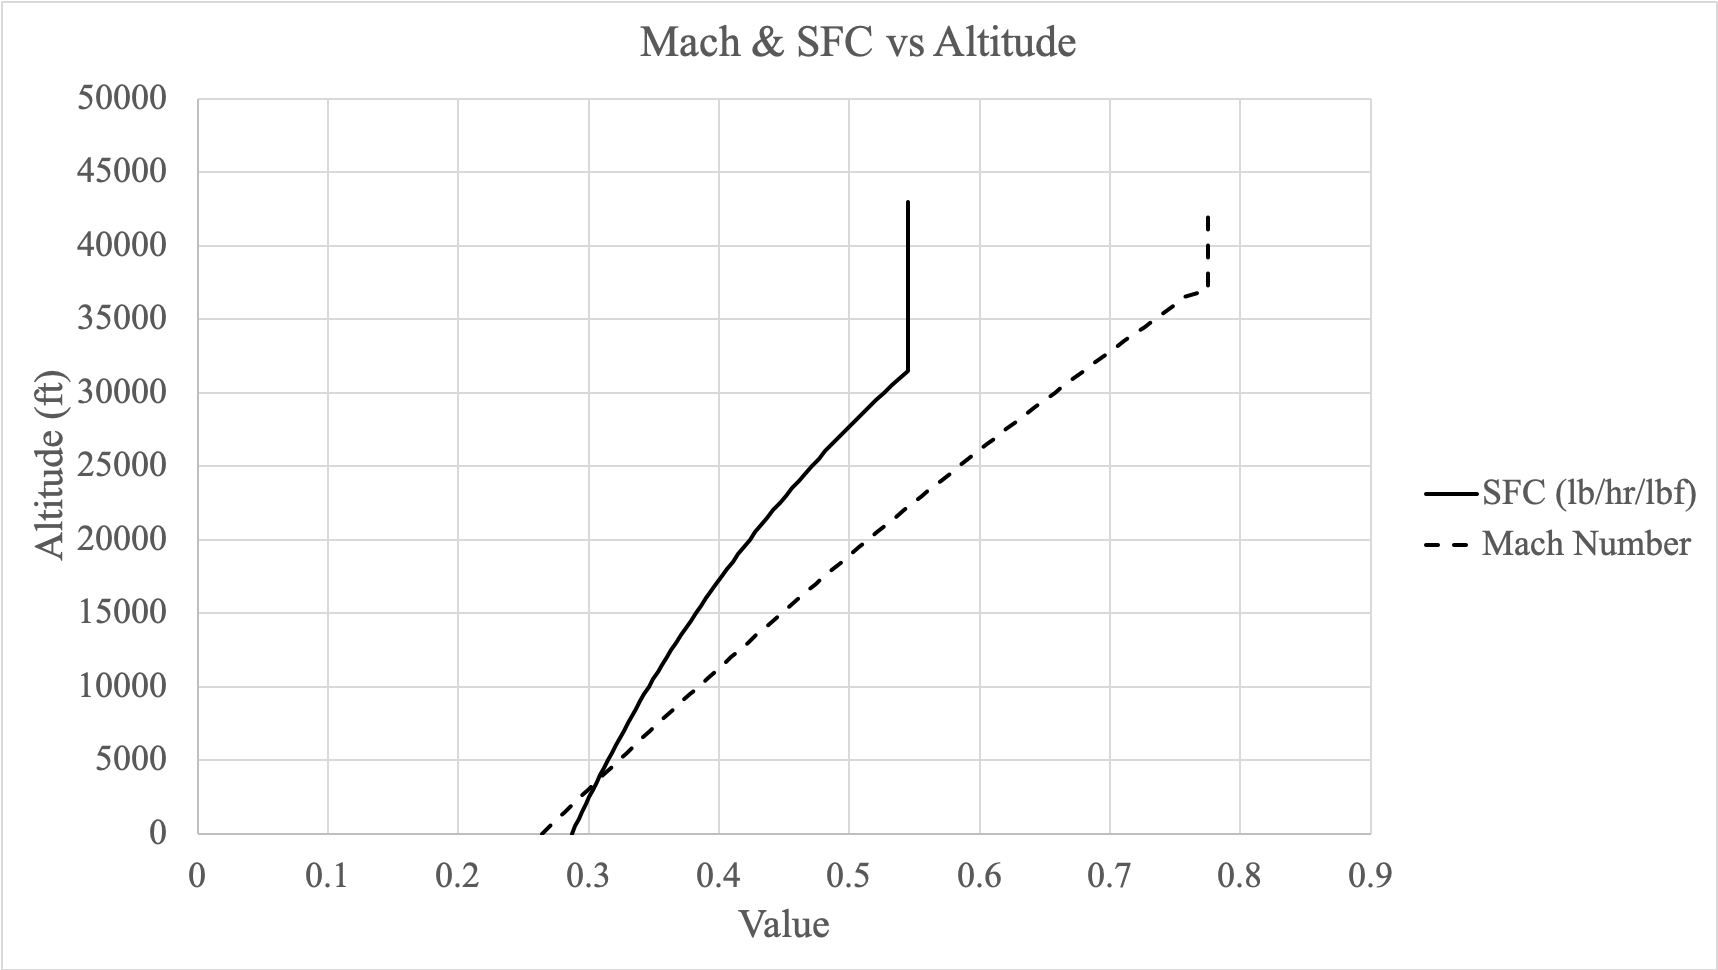
\includegraphics[width=\textwidth]{Photos/propulsion/mach.png}
    \caption{Mach and SFC vs Altitude of the GE90 - 115B}
    \label{fig:machvssfc}
\end{figure}

\begin{figure} [h!]
    \centering
    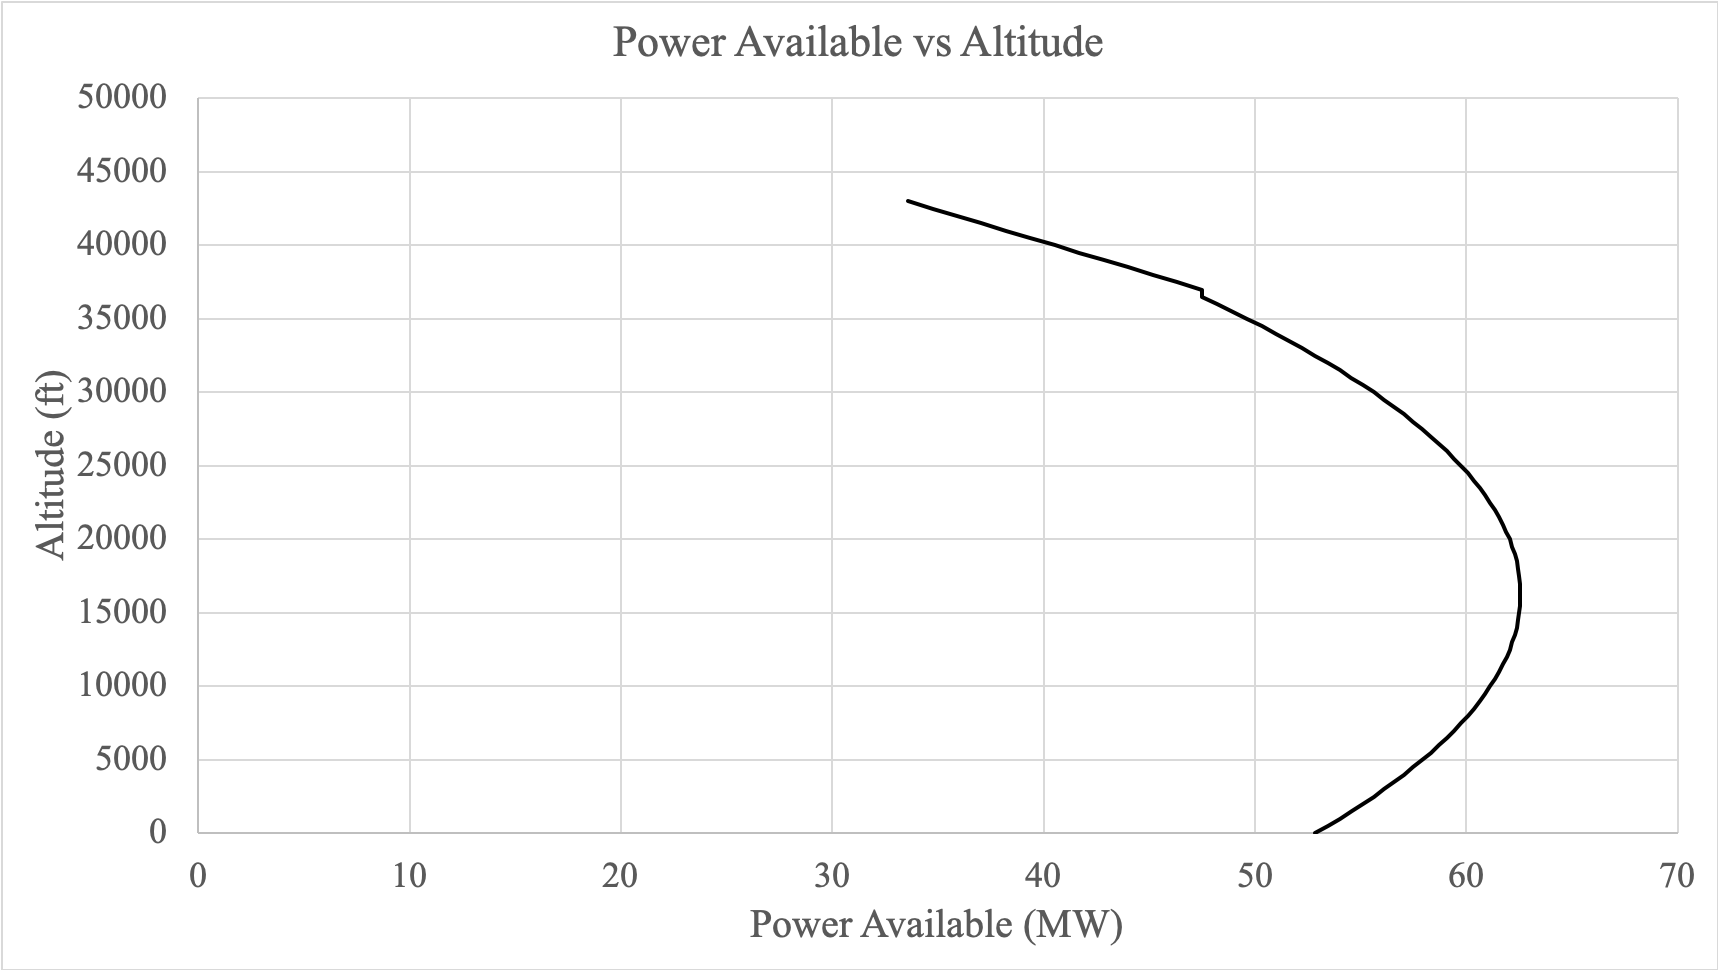
\includegraphics[width=0.8\textwidth]{Photos/propulsion/poweravailable.png}
    \caption{Power Available vs Altitude for the GE90 - 115B}
    \label{fig:poweravailable}
\end{figure}

A trade study was conducted which validated the choice of the GE90-115B. Four main categories were considered: price, SFC, weight and maximum thrust. The maximum thrust and SFC were weighted the heaviest due to the primary driver of reliability and safety. A higher maximum thrust allows greater safety in case one engine fails since the thrust lost will not be as significant. Through all of these considerations, it can be seen that the GE90-115B is the best choice.

\subsection{Inlet, Nacelle/Pod Covers and Exhaust Design}

The engines will be located, one of each side, underneath the wings of the aircraft. This is beneficial for a multitude of reasons, however it is primarily helpful in case of an emergency water landing. Due to the high weight of the engines, when the engines are located under the wing, they will be sheared off on impact during an emergency water landing. With the loss of this heavy, and very dense weight, the aircraft now can float for a longer period of time, allowing passengers more time to reach the safety of lifeboats and evacuate. Other engine mountings were not considered due to noise concerns, controllability and stability concerns in case of engine-out, or due to other safety considerations. Wing mounted engines also have several benefits such as distributing the weight across the wings and the useage of the flaps on the wings can greatly increase lift \cite{raymer}.


The inlet, nacelle cover, and exhaust design were borrowed heavily from the Boeing 777-200, due to the aircraft's similarity to the SAM Mk I. However, some design considerations were taken from Raymer: namely, the nacelle will be angled down by 3 degrees as recommended by \cite{raymer}. In order to have the most efficient turbofan engine as possible, the air entering the engine must be at a Mach of 0.4-0.5 and therefore needs to be slowed down when in flight. This is done by the geometry of the inlet which causes a pressure less and therefore direct increase in the thrust generated by the engine.  The most simple and straightforward inlet is the pitot inlet which would work very well for the SAM Mk I.

\begin{figure} [h!]
    \centering
    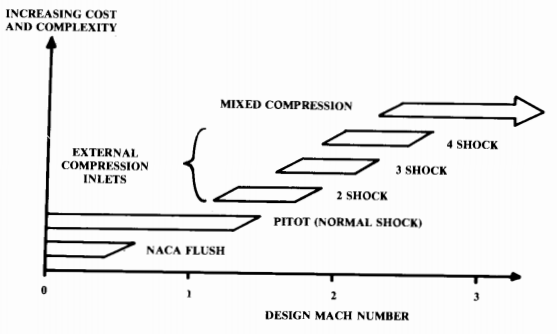
\includegraphics[width=0.8\textwidth]{Photos/inletapplicability.PNG}
    \caption{Inlet Geometry Choice vs Mach}
    \label{fig:inlet}
\end{figure}

Using equations from Raymer, it is possible to determine the capture area of the inlet, and therefore its diameter \cite{raymer}. Using the cruise Mach number of 0.775, the desired Mach number for the air entering the engine of 0.4, compressible flow relations, and the diameter of the GE90-115B of 128 inches, it was calculated that the inlet diameter should be around 79 inches \cite{ge}.

\begin{figure} [h!]
    \centering
    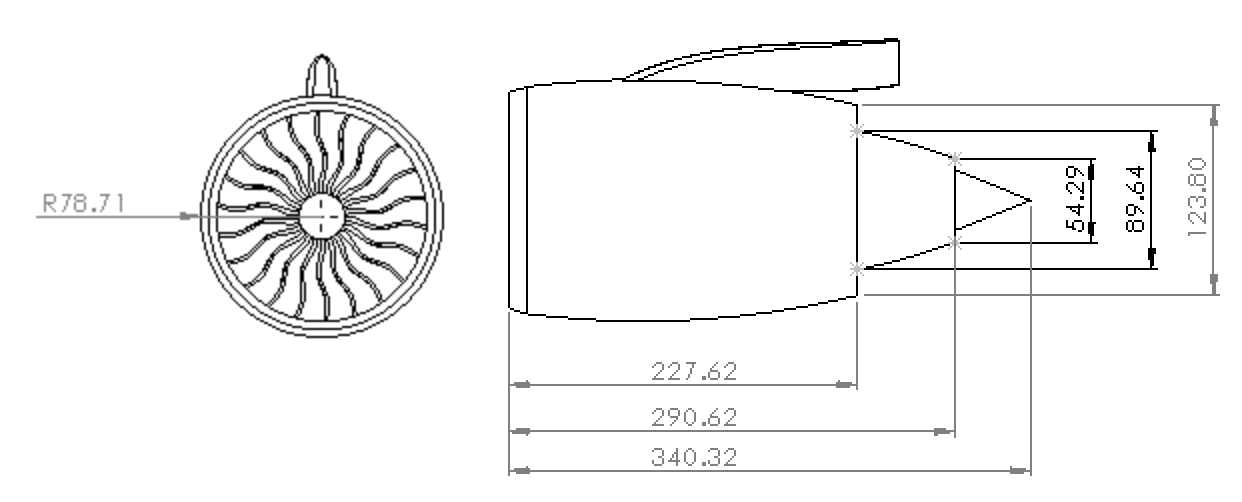
\includegraphics[width=0.8\textwidth]{Photos/propulsion/enginecad.png}
    \caption{Engine CAD in Inches}
    \label{fig:enginecad}
\end{figure}

Similarly, it was possible to estimate the exit area of the engine nozzle using estimation parameters from Raymer. Raymer suggests that the required exit area should be 0.5-0.7 times the inlet area \cite{raymer}. When multiplying the capture area of the inlet area and solving for the radius of the nozzle, it calculates a range of 56 - 66 inches. Therefore, the median value of 61 inches was used in order to estimate an approximate diameter of the exit nozzle as 122 inches.


% \textcolor{red}{
% \begin{itemize}
%     \item AIAA: Propulsion system description and characterization including performance,
%     dimensions, and weights. The selection of the propulsion system(s), sizing, and
%     airframe integration must be supported by analysis, trade studies, and discussion
% \end{itemize}}


% \textcolor{red}{
% \begin{itemize}
%     \item Discuss overall propulsion system design.
%     \begin{itemize}
%         \item Discuss engine requirements (e.g. power and thrust required) and selection.
%         \item Discuss architecture and configuration (e.g. sub-system placement).
%         \item Discuss safety considerations (i.e. engine-out)
%     \end{itemize}
%     \item Discuss main powerplant selected, including decision process, specifications, and performance data (e.g. power available vs altitude vs. Mach, SFC vs. altitude vs. Mach).
%     \item Discuss inlet, nacelle/pod/covers, and exhaust design.
%     \begin{itemize}
%         \item Include basic integration (CAD if using nacelles/pod/covers, general location and spacing if integrated into fuselage).
%         \item Include inlet and exhaust design (e.g. areas, routing).
%         \item Include inlet performance (e.g. pressure losses, install power).
%     \end{itemize}
%     \item Include at least one trade study that uses quantitative or qualitative analysis to support design decisions made.
% \end{itemize}}